\documentclass{beamer}

\usetheme{Warsaw}

\usepackage{verbatim}
\usepackage{xcolor}
\usepackage{listings}
\usepackage{color}
\usepackage[utf8]{inputenc}
\usepackage[T1]{fontenc}
\usepackage{textcomp}
\usepackage{graphicx} 
\usepackage[bulgarian]{babel}
\usepackage{hyperref}
\usepackage{graphicx}

\title{Въведение в Базите данни. Основни понятия и концепции.}
\author{Валентин Гелински}
\institute{ТУ София}
\date{\today} 


\begin{document}
  \begin{frame} 
    \titlepage
  \end{frame}

  \begin{frame}
    \frametitle{За курса}
    \begin{itemize}
      \item{Оценяване}
      \item{Курсови задачи}
    \end{itemize}
  \end{frame}

  \begin{frame}
    \frametitle{Въведение в базите данни}
    \framesubtitle{Или защо си усложняваме живота}
    \begin{itemize}
      \item{Оптимизация по обем (памет)}
      \item{Оптимизация по скорост}
      \item{Консистентност на данните}
      \item{Независимост от кода на програмата}
      \item{Сигурност}
    \end{itemize}
  \end{frame}

  \begin{frame}
    \frametitle{СУБД}
    \framesubtitle{Database Managment System}
    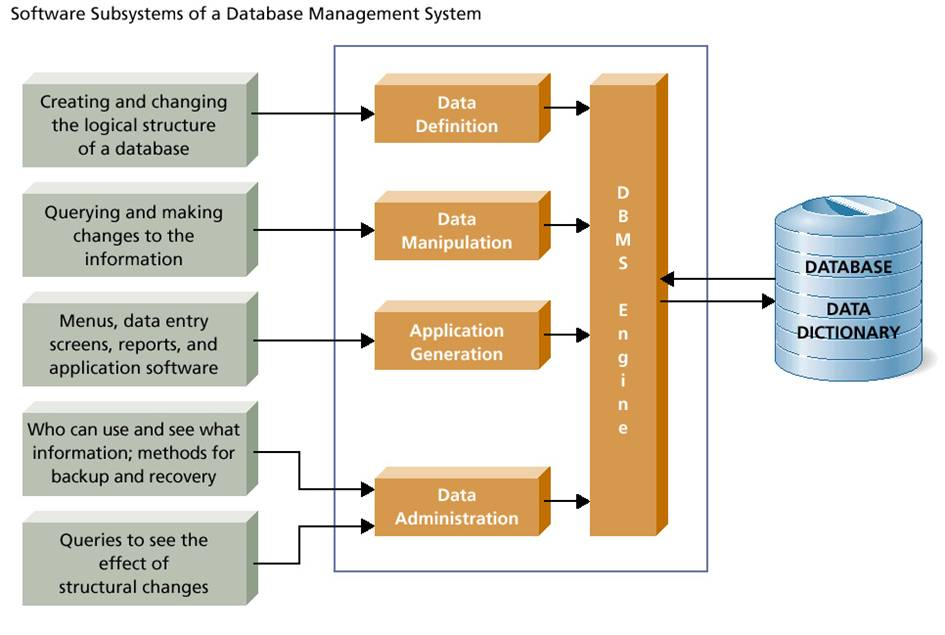
\includegraphics[width=250px]{img/rdbms}
  \end{frame}
\end{document}

